\documentclass[tikz,border=8pt]{standalone}
\usepackage{amsmath,amssymb}
\usetikzlibrary{arrows.meta,calc,positioning}
\begin{document}
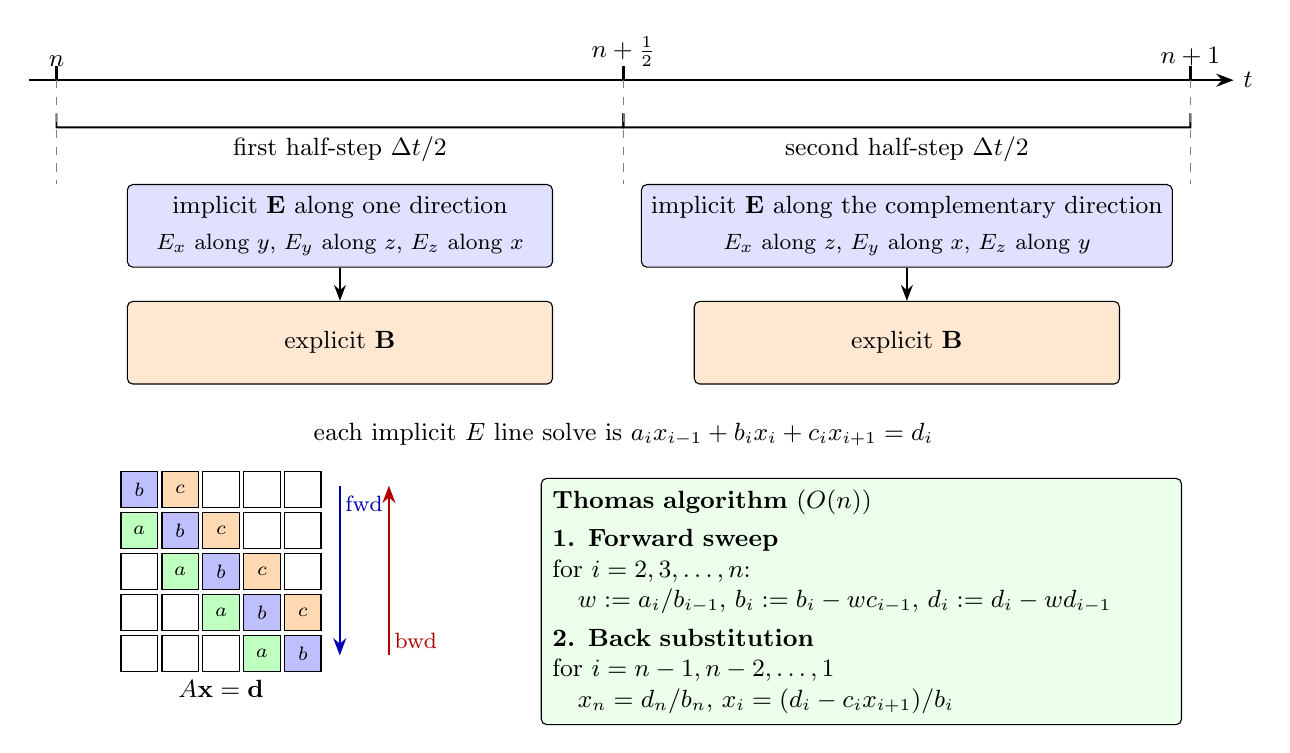
\begin{tikzpicture}[
    font=\small,
    >=Stealth,
    box/.style={draw, rounded corners=2pt, align=center, inner sep=3.5pt, minimum height=1.05cm, minimum width=5.4cm},
    ebox/.style={box, fill=blue!12},
    bbox/.style={box, fill=orange!18},
    tbox/.style={draw, rounded corners=2pt, align=left, inner sep=4pt, fill=green!8},
    cell/.style={draw, minimum size=0.46cm, inner sep=0pt, font=\scriptsize},
]
\def\L{14.4}
\coordinate (O) at (0,0);
\coordinate (M) at (0.5*\L,0);
\coordinate (R) at (\L,0);

% timeline
\draw[-{Stealth[length=2.2mm]}, line width=0.9pt] (-0.35,0) -- (\L+0.55,0);
\foreach \P/\lab in {O/$n$, M/$n+\frac12$, R/$n+1$} {
    \draw[line width=0.9pt] (\P) -- ++(0,0.18);
    \node[above=1.5pt] at (\P) {\lab};
}
\node[right] at (\L+0.55,0) {$t$};

% half-step brackets
\draw[line width=0.7pt] ($(O)+(0,-0.42)$) -- ++(0,-0.18) -- ($(M)+(0,-0.60)$) -- ($(M)+(0,-0.42)$);
\node[below] at (0.25*\L,-0.60) {first half-step $\Delta t/2$};
\draw[line width=0.7pt] ($(M)+(0,-0.42)$) -- ++(0,-0.18) -- ($(R)+(0,-0.60)$) -- ($(R)+(0,-0.42)$);
\node[below] at (0.75*\L,-0.60) {second half-step $\Delta t/2$};

% first half: E above B
\node[ebox] (E1) at (0.25*\L,-1.85) {implicit $\mathbf{E}$ along one direction\\[2pt]
    {\footnotesize $E_x$ along $y$,\ $E_y$ along $z$,\ $E_z$ along $x$}};
\node[bbox, below=0.42cm of E1] (B1) {explicit $\mathbf{B}$};
\draw[-{Stealth[length=2mm]}, thick] (E1) -- (B1);

% second half: E above B (complementary directions)
\node[ebox] (E2) at (0.75*\L,-1.85) {implicit $\mathbf{E}$ along the complementary direction\\[2pt]
    {\footnotesize $E_x$ along $z$,\ $E_y$ along $x$,\ $E_z$ along $y$}};
\node[bbox, below=0.42cm of E2] (B2) {explicit $\mathbf{B}$};
\draw[-{Stealth[length=2mm]}, thick] (E2) -- (B2);

% vertical ticks from timeline to half-step boxes
\draw[dashed, gray] (O) -- (O|-E1.north);
\draw[dashed, gray] (M) -- (M|-E1.north);
\draw[dashed, gray] (R) -- (R|-E2.north);

% ---- tridiagonal / Thomas panel ----
\node[font=\small] at (0.5*\L,-4.50) {each implicit $E$ line solve is $a_i x_{i-1}+b_i x_i+c_i x_{i+1}=d_i$};

% matrix origin
\def\s{0.52}
\coordinate (A0) at (1.05,-5.20);
\foreach \i in {0,1,2,3,4} {
    \foreach \j in {0,1,2,3,4} {
        \node[cell, fill=white] at ($(A0)+(\j*\s,-\i*\s)$) {};
    }
}
% bands: a sub, b diag, c super
\foreach \i in {0,1,2,3,4} {
    \node[cell, fill=blue!25] at ($(A0)+(\i*\s,-\i*\s)$) {$b$};
}
\foreach \i in {0,1,2,3} {
    \node[cell, fill=orange!30] at ($(A0)+({(\i+1)*\s},-\i*\s)$) {$c$};
    \node[cell, fill=green!25] at ($(A0)+(\i*\s,{-(\i+1)*\s})$) {$a$};
}
\node[below=6pt] at ($(A0)+(2*\s,-4*\s)$) {$A\mathbf{x}=\mathbf{d}$};

% both sweep arrows at the right of the matrix
\draw[-{Stealth[length=2.2mm]}, thick, blue!70!black]
    ($(A0)+(4.90*\s,0.05)$) -- ($(A0)+(4.90*\s,-4.05*\s)$);
\node[font=\footnotesize, blue!70!black, anchor=west] at ($(A0)+(4.80*\s,-0.35*\s)$) {fwd};
\draw[-{Stealth[length=2.2mm]}, thick, red!70!black]
    ($(A0)+(6.10*\s,-4.05*\s)$) -- ($(A0)+(6.10*\s,0.05)$);
\node[font=\footnotesize, red!70!black, anchor=west] at ($(A0)+(6.00*\s,-3.70*\s)$) {bwd};

% Thomas steps
\node[tbox, anchor=north west, text width=7.85cm] at (6.15,-5.05) {
    \textbf{Thomas algorithm} ($O(n)$)\\[3pt]
    \textbf{1. Forward sweep} \\
    for $i=2,3,\dots,n$:\\
    \quad $w:=a_i/b_{i-1}$,
    $b_i:=b_i-w c_{i-1}$,
    $d_i:=d_i-w d_{i-1}$\\[3pt]
    \textbf{2. Back substitution}\\
    for $i=n-1,n-2,\dots,1$\\
    \quad $x_n=d_n/b_n$,
    $x_i=(d_i-c_i x_{i+1})/b_i$\\
};
\end{tikzpicture}
\end{document}
